\usepackage{graphicx}%! Author = Philipp Emmenegger
%! Date = 29/06/2021

\subsection{OWASP Mobile Top 10}
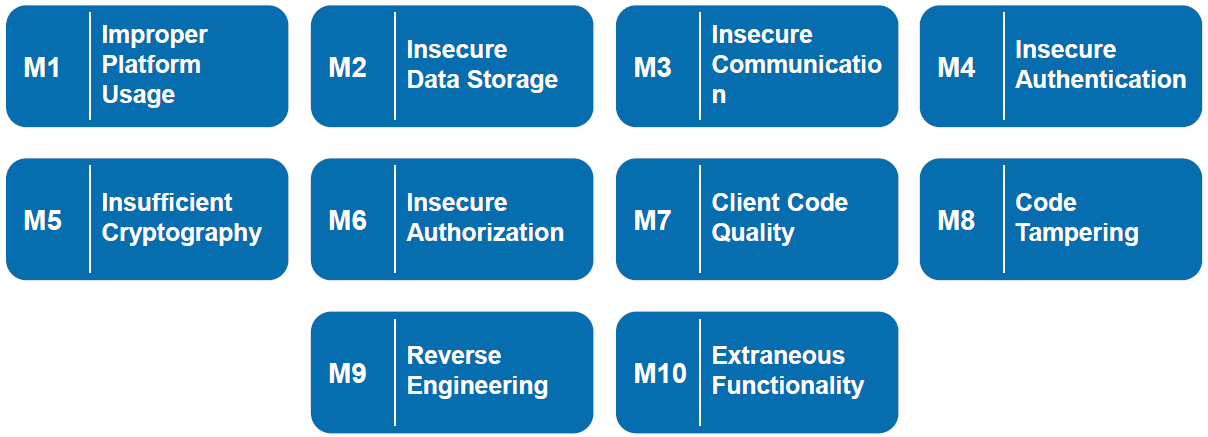
\includegraphics[width=\linewidth]{../img/owasp_mobile.png}

\subsubsection{Improper Platform Usage}
\textbf{Risk}
\begin{itemize}
    \item Violation of published guidelines
    \item Violation of convention or common practice
    \item Unintentional Misuse
\end{itemize}
\textbf{Examples}
\begin{itemize}
    \item Grant app too many permissions
    \item App local Storage Instead of Keychain
\end{itemize}
\textbf{Countermeasures}
\begin{itemize}
    \item Secure coding
    \begin{itemize}
        \item Guidelines by the manufacturer
        \item Best-practices
    \end{itemize}
    \item Secure configuration
    \begin{itemize}
        \item Review
        \item Least privilege
    \end{itemize}
\end{itemize}

\subsubsection{Insecure Data Storage}
\textbf{Risk}
\begin{itemize}
    \item Insecurely storing data
    \begin{itemize}
        \item Databases
        \item Log files
        \item Cookies
        \item SD card
        \item Cloud
    \end{itemize}
    \item Data leakage
    \begin{itemize}
        \item in OS, frameworks, hardware
        \item without developers knowledge
    \end{itemize}
\end{itemize}
\textbf{Channels}
\begin{itemize}
    \item Logs
    \item Screenshots
    \item Keyboard (autocomplete function)
    \item Clipboard
    \item Web Data (Cache, Cookies, Local Storage)
    \item Inter Process Communication
\end{itemize}
\textbf{Countermeasures:}
\begin{itemize}
    \item Critical data
    \begin{itemize}
        \item No logging, no caching
        \item If necessary, mask data
    \end{itemize}
    \item Logs: disable debug logs in production
    \item Keyboard: disable autocomplete
    \item Clipboard: disable copy/paste
    \item Screenshots: use FLAG\_SECURE property
\end{itemize}

\subsubsection{Insecure Communication}
\textbf{Risk}
\begin{itemize}
    \item Cleartext communication of sensitive data
    \item Eavesdropping
    \item TLS/SSL issues
    \item Weak negotiation or ciphers
    \item On any type of communication
\end{itemize}
\textbf{Countermeasures:}
\begin{itemize}
    \item Use SSL/TLS whenever possible
    \item Use good certificates from trusted issuer
    \item Don't send sensitive data over unsecure channels
    \item Certificate Pinning
    \begin{itemize}
        \item Extended validation of SSL server certificate
        \item Store server certificate explicitly in app
        \item Compare on each connection
        \item Certificate renewal must be handled
    \end{itemize}
\end{itemize}

\subsubsection{Insecure Authentication}
\textbf{Risk}
\begin{itemize}
    \item Problems with authentication
    \begin{itemize}
        \item Missing authentication
        \item Weak authentication
        \item Spoofing
        \item Stored passwords
    \end{itemize}
    \item Problems with session management
    \begin{itemize}
        \item Predictable Session ID
        \item No Session Timeout
    \end{itemize}
\end{itemize}
\textbf{Countermeasures}
\begin{itemize}
    \item Authentication
    \begin{itemize}
        \item Perform authentication (also) on server-side
        \item Enforcing strong passwords
        \item Use fingerprint API
    \end{itemize}
    \item Session handling
    \begin{itemize}
        \item Implement session timeout on server side
        \item If data must be stored on client side: encrypted
    \end{itemize}
\end{itemize}

\subsubsection{Insufficient Cryptography}
\textbf{Risk}
\begin{itemize}
    \item Weak ciphers / algorithms
    \item Self made cryptography
    \item Weak keys
    \begin{itemize}
        \item Insufficient length
        \item Stored in an unsecure place
        \item Hardcoded keys
    \end{itemize}
\end{itemize}
\textbf{Countermeasures}
\begin{itemize}
    \item Avoid storing sensitive data on mobile device
    \item Choose proven algorithms / key sizes
    \item Never ever implement crypto yourself
    \item Use hardware-supported crypto
\end{itemize}

\subsubsection{Insecure Authorization}
\textbf{Risk}
\begin{itemize}
    \item Grant access to unauthorized users
    \item Grant operations a user is not entitled for
    \item Examples:
    \begin{itemize}
        \item Insecure Direct Object Reference
        \item Hidden Endpoints (Access to backend API not protected)
    \end{itemize}
\end{itemize}
\textbf{Countermeasures}
\begin{itemize}
    \item Verify roles/permissions on server side
    \item Proper Access control on server side
\end{itemize}

\subsubsection{Client Code Quality}
\textbf{Risk}
\begin{itemize}
    \item Buffer overflows
    \item Format string vulnerabilities
    \item Injection vulnerabilities
    \item XSS
    \item Code executing on the client side
\end{itemize}
\textbf{Countermeasures}
\begin{itemize}
    \item SQL injection: validation, prepared statements
    \item XSS: validation, output encoding
    \item Coding patterns, code analysis tools
    \item Validate length of buffers
    \item Compiler Settings
\end{itemize}

\subsubsection{Code Tampering}
\textbf{Risk}
\begin{itemize}
    \item Counterfeit applications
    \begin{itemize}
        \item re-packaging of original app
        \item malicious code injected
    \end{itemize}
    \item Insecure installation of apps (third party stores)
    \item Techniques:
    \begin{itemize}
        \item Binary patching / monkey patching
        \item Resource patching
        \item Method hooking / swizzling
        \item Jailbreaking / Rooting
    \end{itemize}
\end{itemize}
\textbf{Countermeasures}
\begin{itemize}
    \item Detect code modifications
    \item React to code integrity violations
    \item Jailbreak detection
\end{itemize}

\subsubsection{Reverse Engineering}
\textbf{Risk}
\begin{itemize}
    \item Theft of intellectual property
    \item Disclosure of critical parts
\end{itemize}
\textbf{Countermeasures}
\begin{itemize}
    \item Code Obfuscation
    \item Anti-Debug mechanisms
    \item Use C code
\end{itemize}

\subsubsection{Extraneous Functionality}
\textbf{Risk}
\begin{itemize}
    \item Functionality enabled that was not intended to be released
    \begin{itemize}
        \item Hidden Backdoors
        \item Dev switches
        \item Disabled authentication
    \end{itemize}
    \item Sensitive information
    \begin{itemize}
        \item in comments
        \item in debug logs
    \end{itemize}
\end{itemize}
\textbf{Countermeasures}
\begin{itemize}
    \item Check config files for hidden switches
    \item Make sure dev code is not included into production
    \item Don't put sensitive data into comments
    \item No debug logs in production
    \item Manual secure code review
\end{itemize}

\subsection{Secure Coding Checklist}
\textbf{Data at Rest}
\begin{itemize}
    \item DataProtection API \& Keychain API
    \item Backup Exclusion
    \item Caching
\end{itemize}
\textbf{Data in Motion}
\begin{itemize}
    \item Transport Security
    \item Certificate Pinning
\end{itemize}
\textbf{Data Leakage}
\begin{itemize}
    \item Prevent Side-channel leakage (logs, keyboard, etc.)
\end{itemize}
\textbf{Input Validation}
\begin{itemize}
    \item Input sanitization
    \item Format strings
\end{itemize}
\textbf{Code Protections}
\begin{itemize}
    \item Code Obfuscation
    \item Stack protection
    \item Anti-Debug controls
    \item Compiler settings
    \item Code Injection Checks
\end{itemize}
\textbf{Web-View hardening}
\begin{itemize}
    \item Disable local file access
    \item Disable plugins
    \item Disable JavaScript
    \item URL whitelisting
\end{itemize}
\textbf{Environmental Integrity}
\begin{itemize}
    \item Jailbreak / Rooting detection
    \item Version control / mandatory updates
\end{itemize}